We believe that building models of the world knowledge is a necessary step towards 
operating a workcell in an industrial environment. The proposed models 
for the kitting workstation application include 
representations for non-executable information about the kitting workstation 
such as information about parts, kits, and trays. The description of these 
models includes properties such as the location, orientation, and relation 
between components. These models are discussed in Section~\ref{owlkitting}. 
Models of executable information are also produced from the system 
information described in the SVR. These models include actions along 
with their preconditions, effects, and failures. 
Section~\ref{owlsoap} discusses models of executable information.

Models for non-executable and executable information can be 
combined to generate the OWL/XML kitting \onto{init} and \onto{goal} 
files, as described in Section~\ref{owlinitgoal}.

%+++++++++++++++++++++++++++++++++++++++++++++++++++++++++++%
\subsection{The OWL/XML Kitting Ontology}\label{owlkitting}
%+++++++++++++++++++++++++++++++++++++++++++++++++++++++++++%
In order to maintain compatibility with the IEEE Robotics and 
Automation Society's Ontologies for
Robotics and Automation Working Group, the \onto{Kitting} ontology 
has been fully defined in the Web Ontology Language (OWL)~\cite{OWLoverview}. 
In addition, the ontology was also fully defined in the XML schema 
language~\cite{Walmsley.2002}. Although the two models are 
conceptually identical, there are some systematic differences 
between the models (in addition to differences inherent in 
using two different languages) that are discussed in Balakirsky~\textit{et al.}~\cite{Balakirsky.whitepaper.2012}.
%
%\begin{itemize}
%  \item The \textsf{complexType} names (i.e. class names) in 
%XML schema have the suffix ``Type" added which is not used in OWL. 
%This is so that the same names without the suffix can be used in XML 
%schema language as element names without confusion.
%  \item All of the XML schema \textsf{complexTypes} have a 
%``Name" element that is not present in OWL. It is not needed 
%in OWL because names are assigned as a matter of course when instances of classes are created.
%  \item The XML schema model has a list of ``Object" elements. 
%This collects all of the movable objects. The OWL model does not 
%have a corresponding list. In an OWL data file, the movable objects may appear anywhere.
%  \item OWL has classes but does not have attributes; it has 
%\textsf{ObjectProperties} and \textsf{DataProperties} instead. 
%They may be used to model attributes. OWL Properties are global, 
%not local to a class, so localizing each attribute to a class is 
%done by a naming convention that includes using prefixes as described 
%below. The prefixes are not used in XML schema.
%  \item OWL supports multiple inheritances, but that has not been 
%used in the \onto{Kitting} ontology. Except by subclass relationship, 
%no object is in more than one class.
%\end{itemize}

\begin{table}[h!t!b!]
  \caption{Excerpt of the \onto{Kitting} ontology.}
  \label{tab:kittingonto}
  \centering
  \begin{tabular}{l}
    \hline
    \class{SolidObject} \textit{PrimaryLocation} \textit{SecondaryLocation}
    \\\hline
    \hspace{5 mm}\class{Kit} \textit{Tray} \textit{DesignRef} \textit{Parts} \textit{Finished?}
    \\\hline
    \hspace{5 mm}\class{LargeBoxWithEmptyKitTrays} \textit{LargeContainer} \textit{Trays}
    \\\hline
    \hspace{5 mm}\class{LargeBoxWithKits} \textit{LargeContainer} \textit{Kits} \textit{KitDesignRef} \textit{Capacity}
    \\\hline
    \hspace{5 mm}\class{PartsTrayWithParts} \textit{PartTray}
    \\\hline
    \hspace{5 mm}\ldots
    \\\hline
    \class{DataThing}
    \\\hline
    \hspace{5 mm}\class{PhysicalLocation} \textit{RefObject}
    \\\hline
    \hspace{10 mm}\class{PoseLocation} \textit{Point} \textit{XAxis} \textit{ZAxis}
    \\\hline
    \hspace{15 mm}\class{PoseLocationIn}
    \\\hline
    \hspace{15 mm}\class{PoseLocationOn}
    \\\hline
    \hspace{10 mm}\class{RelativeLocation} \textit{Description}
    \\\hline
    \hspace{15 mm}\class{RelativeLocationIn}
    \\\hline
    \hspace{15 mm}\class{RelativeLocationOn}
    \\\hline
    \hspace{5 mm}\ldots
    \\\hline
  \end{tabular}
\end{table}

\class{SolidObject} and \class{DataThing} constitute the two top-level 
classes of the \onto{Kitting} ontology model, from which all other 
classes are derived. \class{SolidObject} models solid objects, things 
made of matter. The \onto{Kitting} ontology includes several 
subclasses of \class{SolidObject} that are formed from
components that are \class{SolidObject}. The \class{DataThing} 
class models data for \class{SolidObject}. Examples of subclasses 
for \class{SolidObject} and \class{DataThing} are represented in 
Table~\ref{tab:kittingonto}. Items in italics following classes are 
names of class attributes. Derived types inherit the attributes of 
the parent. Each attribute has a specific type not shown in Table~\ref{tab:kittingonto}. 
If an attribute type has derived types, any of the derived types may be used.

Using Table~\ref{tab:kittingonto}, an example of interaction between 
classes \class{SolidObject} and \class{DataThing} can be expressed as 
follows: Each \class{SolidObject} \class{A} has at least one \class{PhysicalLocation} 
(the \textit{PrimaryLocation}). A \class{PhysicalLocation} is defined by 
giving a reference \class{SolidObject} \class{B} (\textit{RefObject}) 
and information saying how the position of \class{A} is related to \class{B}. 
\class{PhysicalLocation} consists of two types of location which are 
required for the operation of the kitting workstation:
\begin{itemize}
 \item Mathematically precise locations are needed to support robot motion. 
The mathematical location, \class{PoseLocation}, gives the pose of the 
coordinate system of \class{A} in the coordinate system of \class{B}. The 
mathematical information consists of the location of the origin of \class{A}'s 
coordinate system (\textit{Point}) and the directions of its Z (\textit{ZAxis}) 
and X (\textit{XAxis}) axes. The mathematical location variety has subclasses 
representing that, in addition, \class{A} is in \class{B} 
(\class{PoseLocationIn}) or on \class{B} (\class{PoseLocationOn}).
\item Relative locations (class \class{RelativeLocation}), 
specifically the knowledge that one \class{SolidObject} is in 
(\class{RelativeLocationIn}) or on (\class{RelativeLocationOn}) 
another, are needed to support making logical plans for building 
kits. The subclasses of \class{RelativeLocation} are needed not only for
logical planning, but also for cases when the relative location is known, but the
mathematical information is not available.
\end{itemize}


%++++++++++++++++++++++++++++++++++++++++++++++++++++++%
\subsection{The OWL/XML SOAP Ontology}\label{owlsoap}
%++++++++++++++++++++++++++++++++++++++++++++++++++++++%
As depicted in Figure~\ref{fig:DesignArchitecture}, the \onto{SOAP} 
ontology imports the \onto{Kitting} ontology. The \onto{Kitting} 
ontology is involved in the process that generates the PDDL domain 
file and in the process that evaluates the truth-value of predicates. 
While some concepts in the \onto{SOAP} ontology are used by both 
processes, other concepts are exclusive to one of these two processes. 
We approach the description of the \onto{SOAP} ontology with a discussion on each process.

%------------------------------------------------------------------------------------------------------------------------------%
\subsubsection{PDDL Domain File Generator Process}\label{sss:domainfile}
%------------------------------------------------------------------------------------------------------------------------------%
A PDDL domain file consists of definitions of predicates, functions, 
and actions. Actions are ways of changing the state of the world and 
consist of a precondition and an effect sections. Predicates and 
functions constitute an action precondition and effect. Predicates 
are used to encode Boolean state variables while functions are used 
to model updates of numerical values. Introducing functions into 
planning makes it possible to model actions in a more compact and 
sometimes more natural way~\cite{FOX.JAIR.2003}. Both predicates 
and functions are well documented in the SVR. 
Figure~\ref{fig:put-part} shows the structure of a domain file.

\begin{figure}[t!h!]
\centering
\begin{minipage}{.5\paperwidth}
\begin{list}{}{\setlength{\leftmargin}{1em}}\item\small
\begin{Verbatim}[commandchars=\\\{\},fontsize=\scriptsize, numbers=left, numbersep=2pt]
(define (domain kitting-domain)
   (:requirements :strips :typing :derived-predicates :action-costs :fluents)
   (:types
      EndEffector
      EndEffectorHolder
      \ldots
   )
(:predicates
   (endeffector-location-robot ?endeffector - EndEffector ?robot - Robot)	
   \ldots
)
(:functions
   (quantity-partstray ?partstray - PartsTray)
   \ldots
)
(:action put-part
   :parameters(
      ?robot - Robot
      ?part - Part
      ?kit - Kit
      ?worktable - WorkTable
      ?partstray - PartsTray)
   :precondition (and
      (part-location-robot ?part ?robot)
      (robot-holds-part ?robot ?part)
      (on-worktable-kit ?worktable ?kit)
      (origin-part ?part ?partstray)
      (< (quantity-kit ?kit ?partstray)
      (capacity-kit ?kit ?partstray))
      (kit-location-worktable ?kit ?worktable))
   :effect (and
      (not (part-location-robot ?part ?robot))
      (not (robot-holds-part ?robot ?part))
      (part-not-searched)
      (not (found-part ?part ?partstray))
      (part-location-kit ?part ?kit)
      (increase (quantity-kit ?kit ?partstray) 1)
      (robot-empty ?robot))
)
\ldots
)
\end{Verbatim}
\end{list}
\end{minipage}
\caption{PDDL action put-part.}
\label{fig:put-part}
\end{figure}
The PDDL domain file consists of a unique name (\texttt{kitting-domain} 
in this example). The \texttt{requirements} section (line 2) 
defines the features that are used in the domain file. The \texttt{types} 
section (lines 3--7) shows the different types of objects that are used 
in predicates, functions, and actions. The \texttt{predicates} section 
(lines 8--11) and the \texttt{functions} section (lines 12--15) list all 
the predicates and functions, respectively, that are used to define an action. 
Both predicates and functions have a unique name, parameters (defined by the 
``?" sign) and types of parameters (placed after the ``-" sign). The \texttt{action} 
section (lines 16--39) formulates the core of an action. The different components 
of an \texttt{action} are described as follows: The unique name of the action 
(\texttt{put-part} in this example) comes directly after the keyword \texttt{:action}. 
The \texttt{parameters} section (lines 17--22) lists all the parameters that 
participate in this action. The \texttt{precondition} section (lines 23--30) 
and the \texttt{effect} section (lines 31--38) list the predicates that must 
be true and the operations on functions.

%\begin{itemize}
%  \item \texttt{action} (line 1): The unique name of the action comes directly after the keyword \texttt{:action}. In this example, the name of the action is \texttt{put-part}.
%  \item \texttt{parameters} (lines 2--7): The parameters (preceded by a ? mark) that participate in this action are listed along their types. For example, line 3 can be read as ``\texttt{robot} is a parameter and is of type \texttt{Robot}''.
%  \item \texttt{precondition} (lines 8--15): List of all the predicates and functions needed in the precondition section.
%  \item \texttt{effect} (lines 16--23): List of all the predicates and functions needed in the effect section.
%\end{itemize}
The automatic generation of a PDDL domain file from the ontology places
certain requirements on the knowledge representation.
It requires class 
definitions of the components described in Figure~\ref{fig:put-part} and the 
definition of the relations between these components. The different classes 
required for the representation of a PDDL domain file are \class{Domain}, 
\class{Predicate}, \class{Function}, \class{Action}, \class{Precondition}, 
\class{Effect}, \class{FunctionBool}, and \class{FunctionOperation}. These 
classes are subclasses of the class \class{DataThing}. The relations between 
these classes are described below.

%
%The representation of PDDL action in the ontology is made up of the classes \class{Action}, \class{Precondition}, \class{Effect}, \class{Predicate}, \class{Function}, \class{ParameterList}.  Operations between functions such as the one shown at lines 28--29 in Figure~\ref{fig:put-part}, are expressed with the class \class{FunctionBool}. All these classes are subclasses of \class{DataThing}.
%
%In the remainder of this section, we provide paragraph descriptions of each of the classes used to represent PDDL actions in the \onto{SOAP} ontology. The naming convention utilized below follows the OWL implementation of the ontology.
\begin{enumerate}
\item \class{Domain} -- A \class{Domain} has a name (\emph{hasDomain\_Name}) of type 
\texttt{string}, at least one requirement (\emph{hasDomain\_Requirement}) of type 
\texttt{string}, and at least a type (\emph{hasDomain\_Type}) of type \texttt{string}. 
A \class{Domain} can consist of 0 or more \class{Predicate} (\emph{hasDomain\_Predicate}) 
and 0 or more \class{Function} (\emph{hasDomain\_Function}). A \class{Domain} has 
at least one \class{Action} (\emph{hasDomain\_Action}).
\item \class{Action} -- An \class{Action} has a unique name (\emph{hasAction\_Name}) of 
type \texttt{string}, a \class{ParameterList} (\emph{hasAction\_ParameterList}) that contains all of the 
parameters for a PDDL action,
a \class{Precondition} (\emph{hasAction\_Precondition}) and 
an \class{Effect} (\emph{hasAction\_Effect}). 
\item \class{ParameterList} -- The \textsl{put-part} action illustrated in 
Figure~\ref{fig:put-part} has five parameters of different types. Each one of 
these types is represented by a class in the \onto{Kitting} ontology. To represent 
all PDDL actions in the \onto{SOAP} ontology, we considered all the different types 
of parameters that are used in all of our ten PDDL actions. To date, we are using eleven 
different types of parameters, represented by the following classes: 
\class{Robot}, \class{EndEffectorChangingStation}, \class{KitTray}, \class{Kit}, 
\class{LargeBoxWithEmptyKitTrays}, \class{LargeBoxWithKits}, \class{WorkTable}, 
\class{PartsTray}, \class{Part}, \class{EndEffector}, and \class{EndEffectorHolder}. 
Therefore, \class{ParameterList} has at least a parameter 
(\emph{hasParameterList\_Parameter}) that is from one of these eleven classes.

    The order of the parameters in a PDDL action also needs to be represented 
in the ontology. In Figure~\ref{fig:put-part}, the parameter \texttt{robot} 
comes before the parameter \texttt{part}, the parameter \texttt{part} comes 
before the parameter \texttt{kit}, and so on. OWL has no built-in structure 
to represent an ordered list. This issue has been solved with the introduction 
of \emph{hasParameter\_Next} that points to the next parameter in \class{ParameterList}.
\item \class{Precondition} -- A \class{Precondition} can consist of \class{Predicate}s 
(\emph{hasPrecondition\_Predicate}) and \class{Function}s (\emph{hasPrecondition\_Function}). 
A \class{Precondition} belongs to one \class{Action} 
(\emph{hadByPrecondition\_Action}).
\item \class{Effect} -- An \class{Effect} can consist of \class{Predicate}s 
(\emph{hasEffect\_Predicate}) and \class{Function}s (\emph{hasEffect\_Function}). 
An \class{Effect} can contain 0 or more \class{FunctionBool} (\emph{hasEffect\_FunctionBool}) 
and 0 or more \class{FunctionOperation}. An \class{Effect} belongs to one \class{Action} 
(\emph{hadByEffect\_Action}). An \class{Effect} can contain negative \class{Predicates} 
which are represented in OWL with the built-in property assertion \texttt{owl:NegativePropertyAssertion}.
\item \class{Predicate} -- A \class{Predicate} has a unique name (\emph{hasPredicate\_Name}) 
of type \texttt{string}. A \class{Predicate} has a reference parameter 
(\emph{hasPredicate\_RefParam}) and a target parameter (\emph{hasPredicate\_TargetParam}). 
A reference parameter is the first parameter in the \class{Predicate}'s list and the target 
parameter is the second parameter in the parameter's list. A \class{Predicate} cannot have 
more than two parameters due to the definition of \class{Predicates} in the SVR. In the 
case a \class{Predicate} has only one parameter, it is assigned to the reference parameter. 
Reference and target parameters refer to the parameters defined in \class{ParameterList} 
for the \class{Action} to which the \class{Predicate} belongs.
\item \class{Function} -- A \class{Function} has a unique name (\emph{hasFunction\_Name}) 
of type \texttt{string}. A \class{Function} has a reference parameter (\emph{hasFunction\_RefParam}) 
and a target parameter (\emph{hasFunction\_TargetParam}). The same rules apply to the 
definition and use of these two types of parameters as the ones described for \class{Predicate}.
\item \class{FunctionBool} -- A \class{FunctionBool} is used to represent functions 
comparison such as the one depicted at lines 28--29 in Figure~\ref{fig:put-part}. 
A \class{FunctionBool} has one or more subclasses that represent the type of relation 
between two \class{Functions}. For example, the relation depicted at lines 28--29 is 
represented in the subclass \class{IntLesserThanInt}. \class{FunctionBool} has a first 
\class{Function} (\emph{hasFunctionBool\_FirstFunction}) that represents the \class{Function} 
on the left side of the operator and a second \class{Function} (\emph{hasFunctionBool\_SecondFunction}) 
that represents the \class{Function} on the right side of the operator.
\item \class{FunctionOperation} -- A \class{FunctionOperation} represents an operation 
on a function such as the one depicted at line 37 in Figure~\ref{fig:put-part}. 
A \class{FunctionOperation} consists of subclasses for each type of operation 
(increase, decrease, \ldots) and \class{FunctionOperation} has one \class{Function} 
(\emph{hasFunctionOperation\_Function}).
\end{enumerate}


%-------------------------------------------------------------%
\subsubsection{The Predicate Evaluation Process}
%-------------------------------------------------------------%
The \process{Predicate Evaluation} process is used to identify action failures 
during plan execution by the robot. The identification of action failures relies 
on spatial relations to compute the truth value of each predicate in each action 
involved in the plan. Action failures and spatial relations are discussed in the remainder of this section.


%-------------------------------------------------------------%
\paragraph{Representation of Action Failure}\label{sss:failure}
%-------------------------------------------------------------%
 A failure is any change or any design or manufacturing error that renders a 
component, assembly, or system incapable of performing its intended function. 
In kitting, failures can occur for multiple reasons: equipment not set up properly, 
tools and/or fixtures not properly prepared, incorrect planning sequence, lack of safety, and improper equipment 
maintenance~\cite{Leger.1999,Kaiser.2007}. Part/component availability failures can be triggered by inaccurate information 
on the location of the part, part damage, wrong type of part, or part shortage due to delays 
in internal logistics. In order to prevent or minimize failures, a disciplined approach 
needs to be implemented to identify the different ways a process design can fail before 
impacting productivity. Failures detected in the workstation can result in the current 
plan becoming obsolete. When a failure is detected in the execution process and the failure 
mode identified, the value of the severity for the failure mode will be retrieved from the 
ontology and the appropriate contingency plan will be activated.
%%%%%%%%%%%%%%%%%%%%%%%%%%%%%%%%%%%%
%%%%%%%%%%% put-part %%%%%%%%%%%
%%%%%%%%%%%%%%%%%%%%%%%%%%%%%%%%%%%%
\begin{table}[h!t!]
  \centering
  \caption{Failure modes for the PDDL action \textsl{put-part}($\mathit{robot}$,$\mathit{part}$,$\mathit{kit}$,$\mathit{worktable}$,$\mathit{partstray}$).}
  \label{tab:putpartfailure}
  \scalebox{0.55}{
  \begin{tabular}{|l|l|l|l|c|c|c|}
    \hline
    \multicolumn{1}{|c|}{\begin{sideways}Action\end{sideways}} &
    \multicolumn{1}{c|}{\begin{sideways}Failure Mode \,\end{sideways}} &
    \multicolumn{1}{c|}{\begin{sideways}Cause \,\end{sideways}} &
    \multicolumn{1}{c|}{\begin{sideways}Effect \,\end{sideways}} &
    \multicolumn{1}{c|}{\begin{sideways}Severity \,\end{sideways}} &
    \multicolumn{1}{c|}{\begin{sideways}Occurrence (\%) \,\end{sideways}} &
    \multicolumn{1}{c|}{\begin{sideways}Predicate \,\end{sideways}} \\
    \hline

    \multirow{6}{*}{\textit{\small{put-part}}} &
    \multirow{2}{*}{\stvar{part} falls off of the end effector} &
    \multirow{2}{*}{end effector hardware issues} &
    downtime & %\stvar{endeffector} replacement &
    9 &
    \multirow{2}{*}{60} &
    \small {\textsf{part-location-robot}}\\\cline{4-5}

     &
     &
     &
    \stvar{part} damage & %\stvar{endeffector} replacement &
    5 &
     &
    \small {\textsf{robot-holds-part}}\\\cline{2-7}

     &
     \multirow{3}{*}{\stvar{part} not released at all}&
     end effector hardware issues &
     downtime &
     9 &
     \multirow{3}{*}{10} &
     $\neg$(\small{\textsf{part-location-robot}})\\\cline{3-5}

     &
     &
     \multirow{2}{*}{wrong/inexistant canonical command} &
     \multirow{2}{*}{downtime} &
     \multirow{2}{*}{7} &
      &
     $\neg$(\small{\textsf{robot-holds-part}})\\
%
     &
     &
     &
     &
     &
     &
     \small {\textsf{robot-empty}}\\\cline{2-7}
     &
     \ldots&
     \ldots&
     \ldots&
     \ldots&
     \ldots&
     \ldots
     \\\hline

\end{tabular}
}
\end{table}
 Table~\ref{tab:putpartfailure} shows an example of failure modes associated with the PDDL 
action \textsl{put-part} where the \textit{Robot} puts the \textit{Part} in the \textit{Kit}. The meaning of each column is described below.



\textit{Action} displays the PDDL action for which failure modes are described and \textit{Failure Mode} lists all possible failure modes that can 
occur during the execution of this action. \textit{Cause} describes the possible root causes for the \textit{Failure Mode}. \textit{Effect} 
displays the effects for each failure mode and it encompasses local and global effects. We note that one failure can have many effects. \textit{Severity} assesses how serious an effect would be should the failure mode occur. Each effect
is given a rank of severity ranging from 1 (minor) to 10 (major). The severity rank will be used in future work to trigger the appropriate contingency plan. \textit{Occurrence} is an estimate
number of frequencies (based on experience) that a failure mode will occur for a specific action. \textit{Predicate} lists the predicates within an action's precondition or effect
that can trigger a failure mode if the truth-values of these predicates are evaluated to false.
%previously presented in Figure~\ref{fig:put-part}.




The classes discussed below are used to represent action failures in the \onto{SOAP} 
ontology and are based on the description of failure modes shown in Table~\ref{tab:putpartfailure}. All these classes are subclasses of the \class{DataThing} class.
\begin{enumerate}
\item \class{Action} -- An \class{Action} has at least one \class{FailureMode} 
(\emph{hasAction\_FailureMode}).
\item \class{FailureMode} -- A \class{FailureMode} has at least one \class{FailureEffect} 
(\emph{hasFailureMode\_FailureEffect}). A \class{FailureMode} has a description 
(\emph{hasFailureMode\_Description}) of type \texttt{Literal} which represents the 
nature of the failure mode. The cause of the failure mode is expressed with 
\emph{hasFailureMode\_Cause} and is of type \texttt{Literal}. The occurrence of 
the failure mode is expressed with \emph{hasFailureMode\_Occurrence} and is of 
type \texttt{Integer}. A \class{FailureMode} has at least one \class{Predicate} 
(\emph{hasFailureMode\_Predicate}) that can trigger the failure mode. The class \class{Predicate} should be represented in the 
ontology \textit{prior} to its association with the class \class{FailureMode}.
\item \class{FailureEffect} -- A \class{FailureEffect} has one failure severity 
(\emph{hasFailureEffect\_FailureSeverity}) of type \texttt{integer} and a 
description (\emph{hasFailureEffect\_Description}) of type \texttt{Literal}.
\end{enumerate}

In the knowledge driven diagram (Figure~\ref{fig:DesignArchitecture}), the 
\process{Predicate Evaluation} process is responsible for failure detection. 
An action failure consists of failure modes that can occur during the execution of a 
PDDL action. The steps to identify action failures in the kitting system are 
described in Figure~\ref{fig:algo}.

\begin{figure}[h!t!]
  \centering
  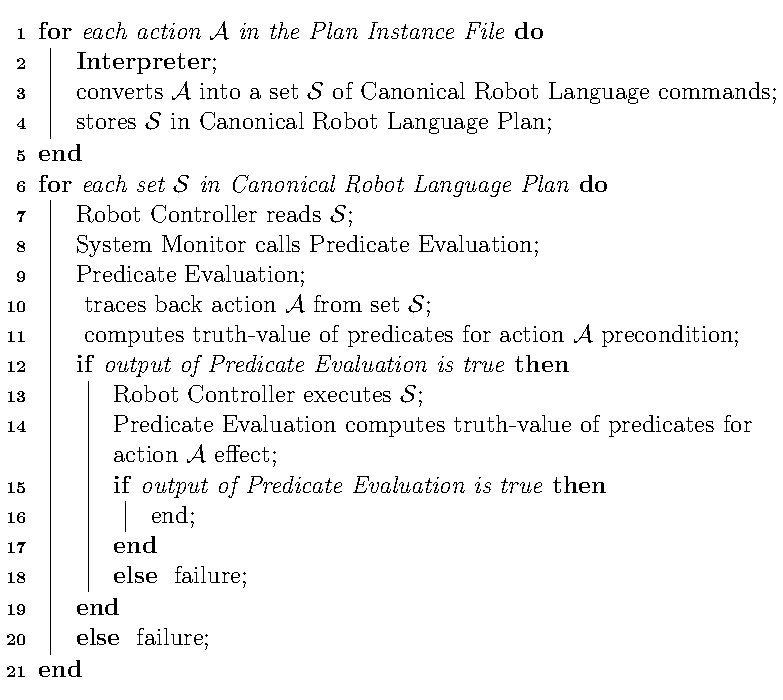
\includegraphics[width=10cm]{images/algorithm.pdf}
  \caption{Failure identification.}
  \label{fig:algo}
\end{figure}

As we can see in Figure~\ref{fig:algo}, failures are identified during the execution of 
canonical robot commands (line 6), generated from PDDL actions (line 3) by the \process{Interpreter}. 
The \process{Predicate Evaluation} process outputs a Boolean value that results in a 
failure detection if this value is false (lines 18 and 20). Once a failure has been 
detected via the \process{Predicate Evaluation} process, the system matches the 
identified failure with one or more failure modes represented in the ontology. The 
following section describes in detail the methodology used by the \process{Predicate Evaluation} 
process to identify failure.


\paragraph{Spatial Relation Representation}
As seen in the previous section, the \process{Predicate Evaluation} process is called by 
the \process{System Monitor} process to check the truth-value of a predicate. The output 
of this process is a Boolean value that is redirected back to the \process{System Monitor}. 
Our kitting system relies on the representation of ``Spatial Relations'' 
to compute the truth-value of each predicate.

``Spatial Relations'' are represented as subclasses of the \class{RelativeLocation} 
class which is a subtype of the \class{PhysicalLocation} (see Table~\ref{tab:kittingonto}). 
There are three types of spatial relations, each represented in a separate class as described below:
\begin{itemize}
 \item \class{RCC8\_Relation}: RCC8~\cite{Wolter.KR.2000} is a well-known and cited 
approach for representing the relationship between two regions in Euclidean space or 
in a topological space. Based on the definition of RCC8, the class \class{RCC8\_Relation} 
consists of eight possible relations, including Tangential Proper Part (TPP), Non-Tangential 
Proper Part(NTPP), Disconnected (DC), Tangential Proper Part Inverse (TPPi), Non-Tangential 
Proper Part Inverse (NTPPi), Externally Connected (EC), Equal (EQ), and Partially 
Overlapping (PO). In order to represent these relations in all three dimensions for the 
kitting domain, we have extended RCC8 to a three-dimensional space by applying it along 
all three planes (x-y, x-z, y-z) and by including cardinal direction relations ``+'' 
and ``-''~\cite{SCHLENOFF.ECDRM.2012}. In the ontology, RCC8 relations and cardinal direction 
relations are represented as subclasses of the class \class{RCC8\_Relation}. Examples of 
such classes are \class{X-DC}, \class{X-EC}, \class{X-Minus}, and \class{X-Plus}.

 \item \class{Intermediate\_State\_Relation}: These are intermediate level state relations 
that can be inferred from the combination of RCC8 and cardinal direction relations. For  
instance, the intermediate state relation \textbf{Contained-In} is used to describe object 
\textit{obj1} completely inside object \textit{obj2} and is represented with the following combination of RCC8 relations:
\begin{gather}
\textbf{Contained-In}(\textit{obj1}, \textit{obj2}) \rightarrow   \notag\\
(\texttt{x-TPP}(\textit{obj1}, \textit{obj2}) \vee \texttt{x-NTPP}(\textit{obj1}, \textit{obj2})) \wedge \notag\\
(\texttt{y-TPP}(\textit{obj1}, \textit{obj2}) \vee \texttt{y-NTPP}(\textit{obj1}, \textit{obj2})) \wedge \notag\\
(\texttt{z-TPP}(\textit{obj1}, \textit{obj2}) \vee \texttt{z-NTPP}(\textit{obj1}, \textit{obj2}))\notag
\end{gather}
In the ontology, intermediate state relations are represented with the OWL built-in property 
\texttt{owl:equivalentClass} that links the description of the class \class{Intermediate\_State\_Relation} 
to a logical expression based on RCC8 relations from the class \class{RCC8\_Relation}.
 \item \class{Predicate}: The representation of predicates has been illustrated in 
Section~\ref{sss:domainfile}. In this section we discuss how the class \class{Predicate} 
has been extended to include the concept of ``Spatial Relation''. The truth-value of 
predicates can be determined through the logical combination of intermediate state relations. 
The predicate \class{kit-location-lbwk}(\textit{kit}, \textit{lbwk}) is true if and only if the 
location of the kit \textit{kit} is in the large box with kits \textit{lbwk}. This predicate can 
be described using the following combination of intermediate state relations:
\begin{gather}
\textsf{kit-location-lbwk}(\textit{kit}, \textit{lbwk}) \rightarrow   \notag\\
\textbf{In-Contact-With}(\textit{kit}, \textit{lbwk}) \wedge \notag\\
\textbf{Contained-In}(\textit{kit}, \textit{lbwk}) \notag
\end{gather}
As with state relations, the truth-value of predicates is captured in the ontology using the 
\texttt{owl:equivalentClass} property that links the description of the class \class{Predicate} 
to the logical combination of intermediate state relations from the class \class{Intermediate\_State\_Relation}.

As seen in Section~\ref{sss:domainfile}, a predicate can have a maximum of two parameters. 
In the case a predicate has two parameters, both parameters are passed to the intermediate 
state relations defined for the predicate, and are in turn passed to the RCC8 relations were 
the truth-value of the predicate is computed. In the case the predicate has only one parameter, 
the truth-value of intermediate state relations, and by inference, the truth-value of RCC8 
relations will be tested with this parameter and with each object in the environment in lieu 
of the second parameter. Our kitting domain consists of only one predicate that has no parameters. 
This predicate is used as a flag in order to force some actions to come before others during the 
formulation of the plan. Predicates of this nature are not treated in the concept of ``Spatial Relation''.
\end{itemize}



%+++++++++++++++++++++++++++++++++++++++++++++++++++++++++++++++++++++++++++++++++%
\subsection{The OWL/XML Kitting Init and Goal Conditions File} \label{owlinitgoal}
%+++++++++++++++++++++++++++++++++++++++++++++++++++++++++++++++++++++++++++++++++%
The OWL/XML kitting \onto{init} and \onto{goal} conditions files are used to build the PDDL 
problem file. This section first describes how a PDDL problem file is structured and then 
reviews the classes used in the different ontologies to build the PDDL problem file.

%-------------------------------------------------%
\subsubsection{Init and Goal sections in the Problem File}
%-------------------------------------------------%
Figure~\ref{fig:problem} is a fragment of the problem file generated for our kitting 
system where we have emphasized the init and goal sections.

\begin{figure}[t!h!]
\begin{minipage}{.7\paperwidth}
\begin{list}{}{\setlength{\leftmargin}{1em}}\item\small
\begin{Verbatim}[commandchars=\\\{\},fontsize=\scriptsize, numbers=left, numbersep=2pt]
(define (problem kitting-problem)
   (:domain kitting-domain)
   (:objects
      robot_1 - Robot
      kit_tray_1 - KitTray
      kit_a2b2c1 - Kit
      \ldots
	)
    (:init
      (robot-with-no-endeffector robot_1)
      (partstray-not-empty part_a_tray)
      \ldots
      (= (capacity-kit kit_a2b2c1 part_a_tray) 2)
      (= (capacity-kit kit_a2b2c1 part_b_tray) 2)
      \ldots)
    (:goal (and
    (= (quantity-kit kit_a2b2c1 part_a_tray) (capacity-kit kit_a2b2c1 part_a_tray))
    \ldots
    (kit-location-lbwk kit_a2b2c1 finished_kit_receiver))
)
\end{Verbatim}
\end{list}
\end{minipage}
\caption{Excerpt of a PDDL problem file for kitting.}
\label{fig:problem}
\end{figure}

The different sections that form the problem file are described as follows. The keyword 
\texttt{problem} (line 1) signals a planner that the current file contains all the elements 
required to constitute a PDDL problem file. The keyword \texttt{domain} (line 2) refers to 
the domain file that the current problem file depends on. The \texttt{objects} section (lines 3--7) 
declares all of the objects present in the world. Some of these objects are required in both the 
initial state and the goal state. The \texttt{init} keyword (line 9) signals a planner about 
the initial state of the world. The predicates that are true and the initial values for 
functions (lines 10--15) are listed in the \texttt{init} section. The \texttt{goal} keyword 
(line 16) signals a planner about the final state of the world. The predicates must be true 
and the functions must have the defined numerical values in this final state.


%------------------------------------------------------------------%
\subsubsection{Representation of the Init and Goal Files Using Ontologies}
%------------------------------------------------------------------%
In our kitting system, the \texttt{init} and \texttt{goal} sections always consist of 
predicates and functions. The following steps describe how we build the OWL/XML kitting 
\onto{init} and \onto{goal} conditions files.
\begin{enumerate}
 \item In the \onto{SOAP} ontology, instances of the objects that will appear in the 
\texttt{objects} section of the problem file are created. Since these objects are used 
in both the \texttt{init} and \texttt{goal} sections in the generated PDDL problem file, 
it is important to make these objects available to the OWL/XML kitting \onto{init} and 
\onto{goal} conditions files. For instance, the object \texttt{robot\_1} of type 
\texttt{Robot} (line 4 in Figure~\ref{fig:problem}) will be generated from the instance 
\texttt{robot\_1} in the class \class{Robot}, created in the \onto{SOAP} ontology.
 \item Predicates and functions that will appear in the \texttt{init} section for the 
generated PDDL problem file are created in the OWL/XML kitting \onto{init} file as instances 
of the class \class{Predicate} and \class{Function}, respectively.
 \item Predicates and functions that will appear in the \texttt{goal} section in the 
generated PDDL problem file are created in the OWL/XML kitting \onto{goal} file as 
instances of the class \class{Predicate} and \class{Function}, respectively.
 \item Instances of the class \class{Predicate} and of the class \class{Function} 
created in the OWL/XML kitting \onto{init} and \onto{goal} conditions files point to parameters (instances of classes) that have been created in the \onto{SOAP} ontology (step 1).
\end{enumerate}


